% Options for packages loaded elsewhere
\PassOptionsToPackage{unicode}{hyperref}
\PassOptionsToPackage{hyphens}{url}
\documentclass[
  11pt,
]{article}
\usepackage{xcolor}
\usepackage[left=2.2cm,right=2.2cm,top=1.8cm,bottom=1.8cm]{geometry}
\usepackage{amsmath,amssymb}
\setcounter{secnumdepth}{5}
\usepackage{iftex}
\ifPDFTeX
  \usepackage[T1]{fontenc}
  \usepackage[utf8]{inputenc}
  \usepackage{textcomp} % provide euro and other symbols
\else % if luatex or xetex
  \usepackage{unicode-math} % this also loads fontspec
  \defaultfontfeatures{Scale=MatchLowercase}
  \defaultfontfeatures[\rmfamily]{Ligatures=TeX,Scale=1}
\fi
\usepackage{lmodern}
\ifPDFTeX\else
  % xetex/luatex font selection
\fi
% Use upquote if available, for straight quotes in verbatim environments
\IfFileExists{upquote.sty}{\usepackage{upquote}}{}
\IfFileExists{microtype.sty}{% use microtype if available
  \usepackage[]{microtype}
  \UseMicrotypeSet[protrusion]{basicmath} % disable protrusion for tt fonts
}{}
\makeatletter
\@ifundefined{KOMAClassName}{% if non-KOMA class
  \IfFileExists{parskip.sty}{%
    \usepackage{parskip}
  }{% else
    \setlength{\parindent}{0pt}
    \setlength{\parskip}{6pt plus 2pt minus 1pt}}
}{% if KOMA class
  \KOMAoptions{parskip=half}}
\makeatother
\usepackage{longtable,booktabs,array}
\newcounter{none} % for unnumbered tables
\usepackage{calc} % for calculating minipage widths
% Correct order of tables after \paragraph or \subparagraph
\usepackage{etoolbox}
\makeatletter
\patchcmd\longtable{\par}{\if@noskipsec\mbox{}\fi\par}{}{}
\makeatother
% Allow footnotes in longtable head/foot
\IfFileExists{footnotehyper.sty}{\usepackage{footnotehyper}}{\usepackage{footnote}}
\makesavenoteenv{longtable}
\usepackage{graphicx}
\makeatletter
\newsavebox\pandoc@box
\newcommand*\pandocbounded[1]{% scales image to fit in text height/width
  \sbox\pandoc@box{#1}%
  \Gscale@div\@tempa{\textheight}{\dimexpr\ht\pandoc@box+\dp\pandoc@box\relax}%
  \Gscale@div\@tempb{\linewidth}{\wd\pandoc@box}%
  \ifdim\@tempb\p@<\@tempa\p@\let\@tempa\@tempb\fi% select the smaller of both
  \ifdim\@tempa\p@<\p@\scalebox{\@tempa}{\usebox\pandoc@box}%
  \else\usebox{\pandoc@box}%
  \fi%
}
% Set default figure placement to htbp
\def\fps@figure{htbp}
\makeatother
% definitions for citeproc citations
\NewDocumentCommand\citeproctext{}{}
\NewDocumentCommand\citeproc{mm}{%
  \begingroup\def\citeproctext{#2}\cite{#1}\endgroup}
\makeatletter
 % allow citations to break across lines
 \let\@cite@ofmt\@firstofone
 % avoid brackets around text for \cite:
 \def\@biblabel#1{}
 \def\@cite#1#2{{#1\if@tempswa , #2\fi}}
\makeatother
\newlength{\cslhangindent}
\setlength{\cslhangindent}{1.5em}
\newlength{\csllabelwidth}
\setlength{\csllabelwidth}{3em}
\newenvironment{CSLReferences}[2] % #1 hanging-indent, #2 entry-spacing
 {\begin{list}{}{%
  \setlength{\itemindent}{0pt}
  \setlength{\leftmargin}{0pt}
  \setlength{\parsep}{0pt}
  % turn on hanging indent if param 1 is 1
  \ifodd #1
   \setlength{\leftmargin}{\cslhangindent}
   \setlength{\itemindent}{-1\cslhangindent}
  \fi
  % set entry spacing
  \setlength{\itemsep}{#2\baselineskip}}}
 {\end{list}}
\usepackage{calc}
\newcommand{\CSLBlock}[1]{\hfill\break\parbox[t]{\linewidth}{\strut\ignorespaces#1\strut}}
\newcommand{\CSLLeftMargin}[1]{\parbox[t]{\csllabelwidth}{\strut#1\strut}}
\newcommand{\CSLRightInline}[1]{\parbox[t]{\linewidth - \csllabelwidth}{\strut#1\strut}}
\newcommand{\CSLIndent}[1]{\hspace{\cslhangindent}#1}
\setlength{\emergencystretch}{3em} % prevent overfull lines
\providecommand{\tightlist}{%
  \setlength{\itemsep}{0pt}\setlength{\parskip}{0pt}}
% Three-part paragraph scaffolding for manuscript revision.
%
% bullets  -- boiled-down topic sentence + bullet points
%             small, sans-serif, dark gray; paragraph number [N] prepended
% rgt      -- author's rewrite (initially a placeholder)
%             small, italic, dark blue
% orig     -- original Claude-authored draft
%             normal size, light gray
%
% Presentation order per paragraph: bullets -> rgt -> orig
% Strip with: strip-claudecode -i report.Rmd

\usepackage{xcolor}

\newcounter{pgraph}

\newenvironment{bullets}{%
  \stepcounter{pgraph}%
  \begin{quote}\small\sffamily\color[gray]{0.30}%
  {\normalfont\scriptsize\color[gray]{0.58}[\thepgraph]\enspace}}{%
  \end{quote}}

\newenvironment{rgt}{%
  \begin{quote}\small\itshape\color[RGB]{20,60,160}}{%
  \end{quote}}

\newenvironment{orig}{%
  \begin{quote}\normalsize\color[gray]{0.55}}{%
  \end{quote}}

% backward compat alias
\newenvironment{claudecode}{\begin{orig}}{\end{orig}}
%% tools/stamp.tex
%% Provenance footer for PDFs rendered from this project.
%% Vendored by zzcollab; this file is not project-specific. The
%% footer prints the source document, the time of rendering, and
%% the git version. All three values are supplied at render time
%% by tools/stamp-render.R, which writes a small generated file
%% that redefines the macros below. The \providecommand defaults
%% keep a bare LaTeX compile working when the document is built
%% without the wrapper.
\usepackage{fancyhdr}
\usepackage{xcolor}
\providecommand{\stampsource}{\detokenize{(source not recorded)}}
\providecommand{\stamptime}{(time not recorded)}
\providecommand{\stampversion}{\detokenize{(version not recorded)}}
\setlength{\footskip}{40pt}
\newcommand{\stampfootcontent}{%
  \footnotesize\color{gray}%
  \parbox[b]{\textwidth}{%
    \stamptime\hfill\thepage\\[2pt]%
    \ttfamily\raggedright\stampsource}}
\pagestyle{fancy}
\fancyhf{}
\fancyfoot[C]{\stampfootcontent}
\renewcommand{\headrulewidth}{0pt}
\renewcommand{\footrulewidth}{0.4pt}
%% The title page uses the `plain` page style; redefine it so the
%% stamp appears there too.
\fancypagestyle{plain}{%
  \fancyhf{}%
  \fancyfoot[C]{\stampfootcontent}%
  \renewcommand{\headrulewidth}{0pt}%
  \renewcommand{\footrulewidth}{0.4pt}}
\renewcommand{\stampsource}{\textasciitilde{}/\allowbreak{}prj/\allowbreak{}res/\allowbreak{}36-pmsimstats-ng/\allowbreak{}pmsimstats-ng/\allowbreak{}analysis/\allowbreak{}report/\allowbreak{}02-carryover-sensitivity/\allowbreak{}report-extra-slim-rgt.Rmd}
\renewcommand{\stamptime}{2026-07-10 00:29 AEST}
\renewcommand{\stampversion}{\detokenize{8d8ea4c-wip}}
\usepackage{amsmath}
\usepackage{amssymb}
\usepackage{setspace}
\setstretch{1.0}
\usepackage{booktabs}
\usepackage{longtable}
\usepackage{array}
\usepackage{multirow}
\usepackage{wrapfig}
\usepackage{float}
\usepackage{colortbl}
\usepackage{pdflscape}
\usepackage{tabu}
\usepackage{threeparttable}
\usepackage{threeparttablex}
\usepackage[normalem]{ulem}
\usepackage{makecell}
\usepackage{xcolor}
\usepackage{bookmark}
\IfFileExists{xurl.sty}{\usepackage{xurl}}{} % add URL line breaks if available
\urlstyle{same}
% fallback for those not using the hyperref driver hyperxmp:
\makeatletter
\@ifundefined{xmpquote}{\newcommand{\xmpquote}[1]{#1}}{}
\makeatother
\hypersetup{
  pdftitle={Exposure-weighted versus lagged-treatment carryover specifications under differential-correlation biomarker interactions: a factorial simulation study},
  pdfauthor={pmsimstats team},
  hidelinks,
  pdfcreator={LaTeX via pandoc}}

\title{Exposure-weighted versus lagged-treatment carryover specifications under differential-correlation biomarker interactions: a factorial simulation study}
\author{pmsimstats team}
\date{2026-07-10}

\begin{document}
\maketitle

\section*{Abstract}\label{abstract}
\addcontentsline{toc}{section}{Abstract}

\textbf{Background.} Aggregated N-of-1 trials pool repeated within-patient
on/off contrasts to validate predictive biomarkers. Under the
multivariate-normal (MVN) differential-correlation architecture
(Architecture B), in which the biomarker-treatment interaction is
encoded in a treatment-state-dependent correlation, a companion study
found that carryover, that is, residual drug effect that decays after
discontinuation, costs up to roughly 31\% of power in relative terms.
The analyst must still decide how to represent residual exposure in
the linear predictor, and it is not established which representation
is most robust to the (typically unknown) pharmacokinetic decay
shape.

\textbf{Methods.} We compare two analysis-model specifications for the
drug-exposure regressor under Architecture B: an exposure-weighted
continuous indicator that assumes a parametric decay and half-life
(A2, the current default), and the binary on-drug indicator augmented
by a lagged just-off-drug term that estimates carryover
non-parametrically (A3, the classical crossover device). We embed
them in an ADEMP-structured factorial simulation\textsuperscript{\citeproc{ref-morris2019simulation}{1}} crossing two data-generating process (DGP)
decay forms (exponential, Weibull) with the two specifications, under
three trial designs, two sample sizes, and three interaction
strengths (216 cells, 500 replicates each), plus four single-axis
sensitivity blocks and a cluster-robust recalibration. Every
performance measure is reported with its Monte Carlo standard error
(MCSE).

\textbf{Results.} A2 attains the highest power only in the two designs
with a blinded-discontinuation phase (Hybrid and OL+BDC), where its
advantage over A3 is about 10 percentage points (0.860 vs 0.770 at
the reference cell). Under the classical crossover (CO) design A2 is
markedly inferior (0.488 vs 0.830 for A3, which tracks the binary
indicator closely). Where A2 leads, the lead is robust to decay-shape
and half-life mis-specification and to autocorrelation strength, and
a paired-McNemar high-precision rerun confirms it is real at the
highest-leverage cell (\(+7.2\) points, \(p = 1.2 \times 10^{-7}\)),
though the two specifications are statistically tied at three of
four other rerun cells. The model-based interaction test is mildly
conservative (mean null rejection 0.039), an artifact of the working
covariance that a CR2 cluster-robust standard error removes without
disturbing the ranking.

\textbf{Conclusions.} Under Architecture B, the exposure-weighted
predictor A2, reported with a cluster-robust standard error, is
recommended for the Hybrid and OL+BDC designs; the lagged-treatment
specification A3 is preferable, or at least not worse, under a
crossover design. Across all conditions, anticipated dropout governs
power far more than the choice between the two specifications, and
should dominate design effort accordingly. This manuscript restricts
the grid to Architecture B and to the exponential and Weibull decay
forms, and does not evaluate the binary on-drug specification (A1)
or Architecture A (mean moderation); the full-scope evaluation,
including those comparisons, is in the companion report.Rmd /
report-slim.Rmd manuscripts.

\section{Introduction}\label{introduction}

In a single N-of-1 trial, one patient is crossed repeatedly between
active treatment and a comparator over a sequence of measurement
occasions, and the within-patient contrast between the on-drug and
off-drug periods estimates that patient's individual treatment
effect. An aggregated N-of-1 trial pools many such single-patient
series into a mixed model, trading some of the resolution available
within a single patient for population-level inference and for
sample sizes considerably smaller than a parallel-group trial would
require\textsuperscript{\citeproc{ref-hendrickson2020}{2}}. The estimand of interest is the
biomarker-treatment interaction, that is, whether a baseline
covariate \(B_i\) modifies the treatment effect. We examine three
trial designs that differ in how the on-drug and off-drug occasions
are arranged, a classical crossover (CO), an open-label design
followed by blinded discontinuation (OL+BDC), and a Hybrid N-of-1
design; each is defined in Section 3.

The inferential complication specific to this setting is carryover.
When a drug is discontinued, its pharmacological effect does not
switch off abruptly but decays over days or weeks, so that
observations recorded during the nominally off-drug period still
carry residual exposure. Treating those observations as though they
were cleanly off-drug mis-specifies the design matrix and attenuates
the interaction test. The question we take up here is which of two
ways of representing residual exposure in the analysis model does
the better job of recovering the power that carryover would
otherwise cost.

A companion study\textsuperscript{\citeproc{ref-pmsimstats_dgp_architectures2026}{3}}, building on
Hendrickson\textsuperscript{\citeproc{ref-hendrickson2020}{2}}, shows that under what we call
Architecture B, a multivariate-normal differential-correlation
formulation in which the interaction lives in the
treatment-state-dependent covariance
\(\text{Cor}(B_i, BR_{it}) = c_{bm} \cdot \phi(t_{sd})\), carryover
erodes power directly: at a half-life of one week, power falls by as
much as roughly 31\% in relative terms, and the loss is strongly
design-dependent, largest under OL+BDC and negligible under CO.
Under an alternative architecture, in which the biomarker instead
moderates the mean response directly, the corresponding loss is only
1 to 3\%; that architecture, together with a third combined
architecture, falls outside the scope of the present manuscript,
which restricts attention to Architecture B, where the carryover
problem is largest and where Hendrickson's original results were
obtained. That earlier work, however, fixed the decay shape at
exponential and evaluated only a single analysis specification,
leaving open the question of which representation of residual
exposure holds up best when the true decay shape is not known with
any precision, as is ordinarily the case in practice.

We compare two ways of representing drug exposure in the linear
predictor: an exposure-weighted continuous indicator that commits to
a parametric decay form and half-life, which we call A2 and which is
the current default in the pmsimstats-ng package, and the binary
on-drug indicator augmented by a lagged just-off-drug term that
estimates the magnitude of carryover without assuming any particular
functional form, which we call A3, following the classical
crossover-trial device described by Jones and Kenward\textsuperscript{\citeproc{ref-jones2014crossover}{4}}. We cross these two specifications against
exponential and Weibull data-generating decay forms and ask whether
one specification can be recommended outright, or whether the choice
depends on the trial design. The study follows the ADEMP reporting
framework of Morris, White, and Crowther\textsuperscript{\citeproc{ref-morris2019simulation}{1}}, and every performance measure we report
carries its Monte Carlo standard error. Section 3 describes the
simulation design in ADEMP order, Section 4 gives the results, and
Section 5 takes up the practical implications for trialists.

\section{Simulation design}\label{simulation-design}

\subsection{Aims}\label{aims}

The aim of this study is to quantify, under Architecture B, the cost
of mis-specifying the carryover representation in the analysis
model, and to determine which of the two candidate strategies, A2 or
A3, holds up better across the grid of data-generating decay forms
and trial designs. A second and related aim, addressed in the Tier 2
sensitivity blocks of Section 4, is to check whether the resulting
ranking survives perturbation of the within-subject autocorrelation,
the dropout rate, the accuracy of the assumed half-life, and the
size of the biomarker-treatment interaction itself.

\subsection{Data-generating mechanism}\label{data-generating-mechanism}

Under Architecture B, the biomarker and the biological response are
drawn jointly from a multivariate normal distribution with a
treatment-state-dependent correlation,
\(\text{Cor}(B_i, BR_{it}) = c_{bm} \cdot \phi(t_{sd})\), where \(\phi\)
denotes the decay form and \(t_{sd}\) is the time elapsed since drug
discontinuation. Architecture A, in which the biomarker instead
moderates the mean response directly, and a combined Architecture C,
fall outside the scope of the present manuscript; the full
comparison across architectures is reported in the companion
report.Rmd and report-slim.Rmd manuscripts. In both architectures,
the decay function \(\phi : \mathbb{R}_+ \to [0, 1]\) maps \(t_{sd}\) to
a residual-effect multiplier. We evaluate two such forms here, each
parameterized to match a common half-life \(t_{1/2}\). A third form,
linear decay, appears in the full-scope manuscripts but is not
considered further here.

\subsubsection{Exponential decay}\label{exponential-decay}

\[
\phi_{\text{exp}}(t_{sd}) =
  \exp\left(-\lambda t_{sd}\right), \qquad
  \lambda = \frac{\ln 2}{t_{1/2}}
\]

This is the decay form used throughout the companion manuscript, and
it is the one currently implemented in
\texttt{implementations/tidyverse/R/functions.R}. It corresponds to
classical first-order elimination kinetics and is the default
assumption in pharmacokinetics, and we retain it here as the
reference against which the Weibull form is compared.

\subsubsection{Weibull decay}\label{weibull-decay}

\[
\phi_{\text{weib}}(t_{sd}) =
  \exp\left(-\left(\lambda_w t_{sd}\right)^{k}\right), \qquad
  \lambda_w = \frac{(\ln 2)^{1/k}}{t_{1/2}}
\]

A shape parameter \(k\) governs whether the elimination tail is
heavier than exponential (\(k < 1\), slower elimination) or lighter
(\(k > 1\), faster off-drug clearance); the exponential form is
recovered exactly at \(k = 1\). We report results at \(k = 0.7\),
representing a drug with a prolonged low-concentration tail, and at
\(k = 1.5\), representing a drug cleared more rapidly once
concentration falls below some saturation threshold, perhaps through
active transport. Together with \(k = 1.0\), which is numerically
indistinguishable from the exponential form, this gives four
decay-shape levels in the grid.

\subsection{Estimand and analysis specifications}\label{estimand-and-analysis-specifications}

Under Architecture B, the interaction estimand is the on-drug
biomarker-response correlation \(c_{bm}\), a dimensionless quantity.
Bias and empirical standard error are reported on a calibrated
effect-size scale, namely the expected difference in on-drug
response per standard deviation of the biomarker at \(t_{1/2} = 0\),
as defined in \texttt{docs/19-mean-moderation-implementation-notes.tex};
power and Type I error are reported on the native test-statistic
scale. The null estimand used for Type I error verification is
\(c_{bm} = 0\), realized by the corresponding row of the parameter
grid.

The analysis model is \texttt{nlme::lme(Sx\ \textasciitilde{}\ bm\ *\ X\ +\ t,\ random\ =\ \textasciitilde{}1\ \textbar{}\ ptID,\ correlation\ =\ corCAR1(form\ =\ \textasciitilde{}\ t\ \textbar{}\ ptID))} for both
specifications considered here; they differ only in how the
drug-exposure predictor \(X\) is constructed.

\subsubsection{A2: exposure-weighted (continuous predictor)}\label{a2-exposure-weighted-continuous-predictor}

Under A2, \(X = \text{Dbc}_{it}\), a continuous exposure-decayed
predictor constructed to match the analyst's assumed decay form and
half-life; this is the current pmsimstats-ng default. At on-drug
timepoints \(D_{bc,it} = 1\) regardless of the assumed half-life. At
off-drug timepoints the predictor decays as
\(D_{bc,it} = \exp(-(\ln 2/\hat{t}_{1/2})\,t_{sd,it}) =
(1/2)^{t_{sd,it}/\hat{t}_{1/2}}\), losing exactly half its value for
every \(\hat{t}_{1/2}\) weeks that elapse after discontinuation. When
the analyst's assumed decay form matches the true data-generating
form, the predictor is well matched; when it does not, it is
mis-specified in a way we probe directly in Tier 2 block S2. It is
worth noting that the half-life assumption enters only through the
predictor values handed to \texttt{lme}, not through the model formula,
which is identical regardless of \(\hat{t}_{1/2}\); A2 is, in effect,
a different model for every value of the assumed half-life, even
though it is written the same way each time.

\subsubsection{A3: lagged-treatment (estimated carryover term)}\label{a3-lagged-treatment-estimated-carryover-term}

Under A3, \(X = D_{it}\) is augmented with a lagged-treatment indicator
\(L_{it} = D_{i,t-1}(1 - D_{it})\), which marks the off-drug timepoints
immediately following an on-drug timepoint. The magnitude of
carryover is estimated from the data rather than assumed in advance,
so this specification does not require the analyst to posit any
particular decay form. The device follows the classical
crossover-trial tradition surveyed by Jones and Kenward\textsuperscript{\citeproc{ref-jones2014crossover}{4}}. One structural feature of A3 is worth
flagging, since it bears directly on how the results should be read:
the lagged term \(L_{it}\) enters the model only as a nuisance main
effect, and the interaction actually tested under A3 remains
\(\text{bm:}D_{it}\), the same coefficient tested under the binary
on-drug specification (which we call A1 and do not evaluate further
in this manuscript). A3 is best understood, then, as A1 with a
carryover nuisance control added, rather than as a fundamentally
different model of the interaction. Because it carries no half-life
parameter, A3 is invariant to the analyst's assumed half-life by
construction, in contrast to A2, and this asymmetry, one
specification indexed continuously by \(\hat{t}_{1/2}\) and the other
not a member of that family at all, is what the Tier 2 block S2
sensitivity contrast in Section 4.5 is designed to probe.

\subsection{Factorial grid and parameter settings}\label{factorial-grid-and-parameter-settings}

The principal comparison is a factorial of DGP decay form (four
levels: exponential; Weibull at \(k \in \{0.7, 1.0, 1.5\}\)) against
analysis-model specification (A2, A3), under Architecture B only:

\begin{table}

\caption{\label{tab:grid-table}Principal simulation grid (Architecture B only). Cell 1
    is the matched reference: exponential DGP analyzed under the
    current pmsimstats-ng default. Off-diagonal cells quantify the
    cost of DGP-analysis mis-specification.}
\centering
\begin{tabular}[t]{l|l|l}
\hline
DGP decay & A2 exposure-weighted & A3 lagged-treatment\\
\hline
Exponential & cell 1 (matched) & cell 2\\
\hline
Weibull (k = 0.7) & cell 3 & cell 4\\
\hline
Weibull (k = 1.0) & cell 5 & cell 6\\
\hline
Weibull (k = 1.5) & cell 7 & cell 8\\
\hline
\end{tabular}
\end{table}

{\def\LTcaptype{none} % do not increment counter
\begin{longtable}[]{@{}ll@{}}
\toprule\noalign{}
Parameter & Values \\
\midrule\noalign{}
\endhead
\bottomrule\noalign{}
\endlastfoot
Biomarker moderation (\(c_{bm}\)) & 0.0, 0.30, 0.45 \\
Carryover half-life (\(t_{1/2}\)) & 0.0, 0.5, 1.0 weeks \\
Weibull shape (\(k\)) & 0.7, 1.0, 1.5 (Weibull form only) \\
Sample size (\(N\)) & 35, 70 \\
Trial design & CO, N-of-1 (Hybrid), OL+BDC \\
DGP architecture & B (MVN differential correlation) only \\
Replicates per cell & 500 (target); 50 for development \\
\end{longtable}
}

The 216-cell count follows the same nesting logic used in the
full-scope manuscript, with the architecture dimension fixed at B
and the linear decay form removed. The decay-shape combinations
number four (exponential, and Weibull at \(k \in \{0.7, 1.0, 1.5\}\)),
so the grid comes to \(4 \times 3 \times 3 \times 2 \times 3 = 216\)
cells, the factors being decay shape, carryover half-life, trial
design, sample size, and biomarker level. The \(c_{bm} = 0\) row
serves as the Type I error check, targeting the nominal 5\% level,
and the \(t_{1/2} = 0\) row, in which carryover is absent altogether,
gives a best-case power reference at each combination of sample
size, design, and \(c_{bm}\), against which the power cost of nonzero
carryover can be read off directly.

\subsection{Performance measures and computing environment}\label{performance-measures-and-computing-environment}

For each cell we report Power, Type I error (at \(c_{bm} = 0\)), Bias
and Empirical SE of the interaction estimate (on the calibrated
scale), Coverage of the nominal 95\% Wald CI, MSE, the
non-convergence rate, and the MCSE of each measure, following Morris
et al.\textsuperscript{\citeproc{ref-morris2019simulation}{1}, Tables 5-6}.

We chose \(n_{sim} = 500\) so that the Monte Carlo standard error on
power at \(p = 0.5\) would not exceed 0.022
(\(\sqrt{0.5 \cdot 0.5 / 500} \approx 0.022\)). No simulation is run
for this manuscript; we instead filter the same production-scale
grid summary used in the full-scope report.Rmd and report-slim.Rmd
manuscripts (540 cells, \texttt{analysis/data/02-grid-summary.rds},
computed with \texttt{implementations/tidyverse/} as the primary
implementation under R 4.5.3, 128 minutes on eight cores, commit SHA
\texttt{7018b59}, dated 2026-04-15) down to the 216-cell slice defined by
Architecture B, the two non-linear decay forms, and the A2 and A3
specifications. Within each cell, both remaining specifications were
fit to the same simulated dataset (common random numbers), so the
A2 minus A3 contrast is estimated with reduced Monte Carlo variance
relative to what independent draws would give. The Tier 2
sensitivity blocks and the S6 cluster-robust recalibration are
filtered from the same shared outputs
(\texttt{analysis/data/02-sensitivity-summary.rds} and
\texttt{analysis/scripts/carryover-sensitivity/output/diag-s6-cr2.rds});
their designs were already anchored at Architecture B. The filtered
figures used here are produced by \texttt{03-render-figures-extra-slim.R},
\texttt{04-sensitivity-figures-extra-slim.R}, and
\texttt{07-type1-cr2-figure-extra-slim.R}.

\section{Results}\label{results}

All results reported below derive from the same 500-replicate
production run used in the full-scope manuscripts, filtered to
Architecture B, the exponential and Weibull decay forms, and the A2
and A3 specifications. The Monte Carlo standard error on power does
not exceed 0.022 at \(p = 0.5\), and differences smaller than this
should not be over-interpreted. Coverage of the nominal 95\% Wald
confidence interval is reported for the reference cell, and
non-convergence rates are reported per cell in the tables that
follow.

\subsection{Headline performance table}\label{sec-headline}

Table \ref{tab:headline} reports performance at the reference cell
(Architecture B, exponential DGP, Hybrid design, \(N = 70\),
\(c_{bm} = 0.45\)), where non-convergence was zero throughout. A
caveat applies to the bias, mean squared error, and coverage
columns: these are computed against A2's calibrated target,
\(\theta_{\text{true}} = -c_{bm}\sigma_{BR} = -3.6\), while A3
estimates a different coefficient, \(\text{bm:}D_{it}\). A3's apparent
bias and under-coverage in this table reflect that mismatch in
estimand rather than any defect in the estimator, and for that
reason we compare only power and Type I error across the two
specifications; the bias and coverage columns are reported for
completeness but are not directly comparable between A2 and A3.

\begin{table}

\caption{\label{tab:headline}Headline performance at the reference cell
    (Architecture B, exponential DGP, Hybrid design, $N = 70$,
    $c_{bm} = 0.45$, $n_{sim} = 500$). Power is the rejection rate of
    $H_0: \beta_{bm:X} = 0$ at $\alpha = 0.05$. Bias is on the
    calibrated effect-size scale,
    $\theta_{\text{true}} = -c_{bm} \cdot \sigma_{BR} = -3.6$
    (per docs/19 calibration). MCSEs are reported per Morris et al.
    (2019, Table 6).}
\centering
\begin{tabular}[t]{rlllllll}
\toprule
t1/2 & spec & Power (MC SE) & Bias (MC SE) & Empirical SE & Coverage (MC SE) & MSE (MC SE) & Non-conv\\
\midrule
0.0 & A2 & 0.988 (0.005) & -0.029 (0.033) & 0.746 & 0.990 (0.004) & 0.557 (0.034) & 0.000\\
0.0 & A3 & 0.990 (0.004) & -0.025 (0.033) & 0.746 & 0.990 (0.004) & 0.557 (0.034) & 0.000\\
0.5 & A2 & 0.948 (0.010) & +0.072 (0.041) & 0.907 & 0.972 (0.007) & 0.828 (0.057) & 0.000\\
0.5 & A3 & 0.920 (0.012) & +0.583 (0.036) & 0.812 & 0.938 (0.011) & 1.000 (0.059) & 0.000\\
1.0 & A2 & 0.860 (0.016) & -0.081 (0.049) & 1.085 & 0.968 (0.008) & 1.184 (0.077) & 0.000\\
\addlinespace
1.0 & A3 & 0.770 (0.019) & +1.099 (0.038) & 0.853 & 0.818 (0.017) & 1.935 (0.094) & 0.000\\
\bottomrule
\end{tabular}
\end{table}

\subsection{Matched-decay baseline}\label{matched-decay-baseline}

At the matched cell (exponential DGP, A2 exposure-weighted analysis,
Architecture B, \(N = 70\), \(c_{bm} = 0.45\), Hybrid design), power
declines from \(0.988 \pm 0.005\) at \(t_{1/2} = 0\) to
\(0.948 \pm 0.010\) at \(t_{1/2} = 0.5\) to \(0.860 \pm 0.016\) at
\(t_{1/2} = 1.0\) weeks (point estimate plus or minus MCSE,
\(n_{sim} = 500\)). All 500 replicates converged at every half-life in
this cell. The value at \(t_{1/2} = 1.0\) agrees with Hendrickson's
reported power of 0.82 for the same cell\textsuperscript{\citeproc{ref-hendrickson2020}{2}}, which
we take as reassurance that the simulation pipeline reproduces the
baseline result correctly.

\subsection{Power by analysis specification}\label{power-by-analysis-specification}

\begin{figure}
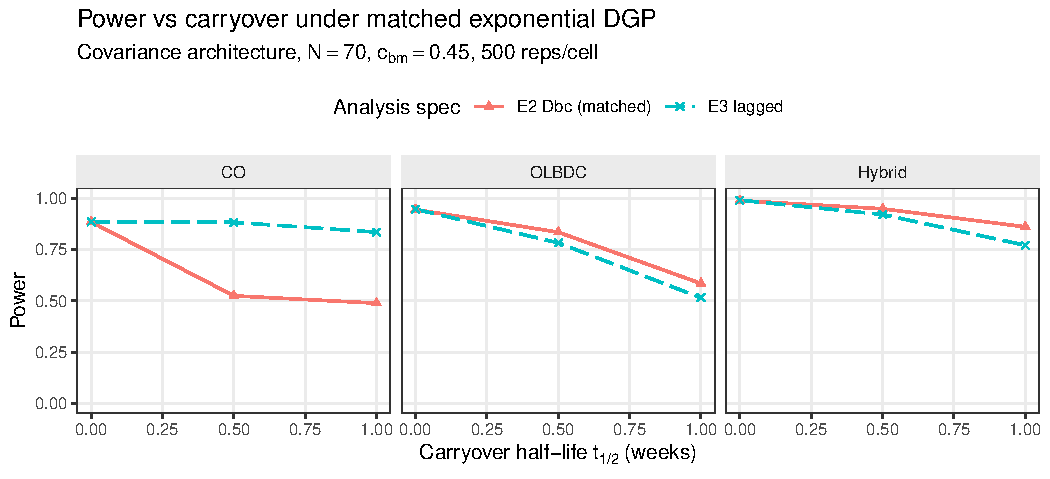
\includegraphics[width=0.95\linewidth]{../../figures/02xs-power-by-spec} \caption{Power versus carryover half-life under the exponential DGP, Architecture B, stratified by analysis specification. A2 retains a modest advantage over A3 in the Hybrid and OL+BDC designs at $t_{1/2} = 1.0$ weeks, but is dominated by A3 under the crossover (CO) design.}\label{fig:fig-power-by-spec}
\end{figure}

The two specifications give nearly identical power at \(t_{1/2} = 0\),
where there is no carryover to model, and diverge progressively as
the half-life increases. A2 retains a modest but consistent
advantage in the Hybrid and OL+BDC designs, an advantage that first
appears at \(t_{1/2} = 0.5\) weeks and grows through \(t_{1/2} = 1.0\)
weeks. This advantage does not appear under the crossover design,
where A2 is in fact dominated, a point we return to in Section 5.
The mechanism is fairly clear: in a crossover trial, the
within-subject correlation already carries most of the signal that
A2's decaying predictor was designed to recover, so A2 has little
left to gain, and its down-weighting of the off-drug observations
only works against it.

\subsection{Decay-form mis-specification}\label{decay-form-mis-specification}

\begin{figure}
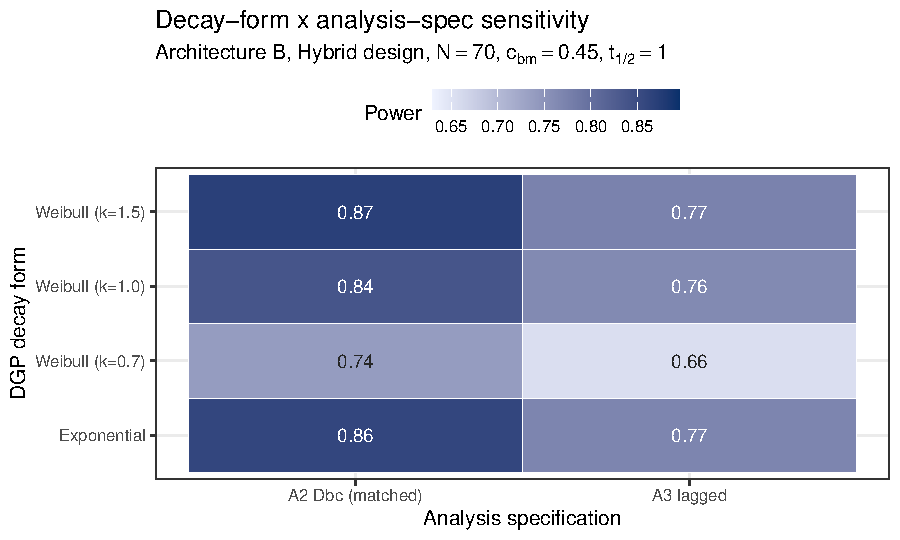
\includegraphics[width=0.7\linewidth]{../../figures/02xs-heatmap-matched-vs-mismatched} \caption{Power at the critical cell ($t_{1/2} = 1.0$ weeks, Architecture B, Hybrid design, $N = 70$, $c_{bm} = 0.45$) across DGP decay forms (rows) and analysis specifications (columns). Under the heavy-tailed Weibull DGP ($k = 0.7$), A2's advantage over A3 narrows because its assumed exponential decay no longer matches truth. The fill scale is stretched to the observed power range (0.66-0.87), not the full [0,1] range, so that these cell-to-cell differences are visible; the absolute shading should not be compared to other figures in this manuscript.}\label{fig:fig-heatmap-mismatch}
\end{figure}

The heatmap cell at the intersection of the exponential DGP row and
the A2 column is the matched reference, with power
\(0.860 \pm 0.016\). The same row's A3 column gives the power penalty
of the lagged specification when the data-generating decay is
exponential, while the other rows of the A2 column give the cost of
assuming exponential decay in the analysis when the true decay form
is Weibull. Even under the heaviest-tailed Weibull data-generating
process we examined (\(k = 0.7\)), A2's advantage over A3 narrows but
does not reverse. We take up the practical interpretation of this in
Section 5.

\subsection{Type I error control and cluster-robust recalibration}\label{type-i-error-control-and-cluster-robust-recalibration}

\begin{figure}
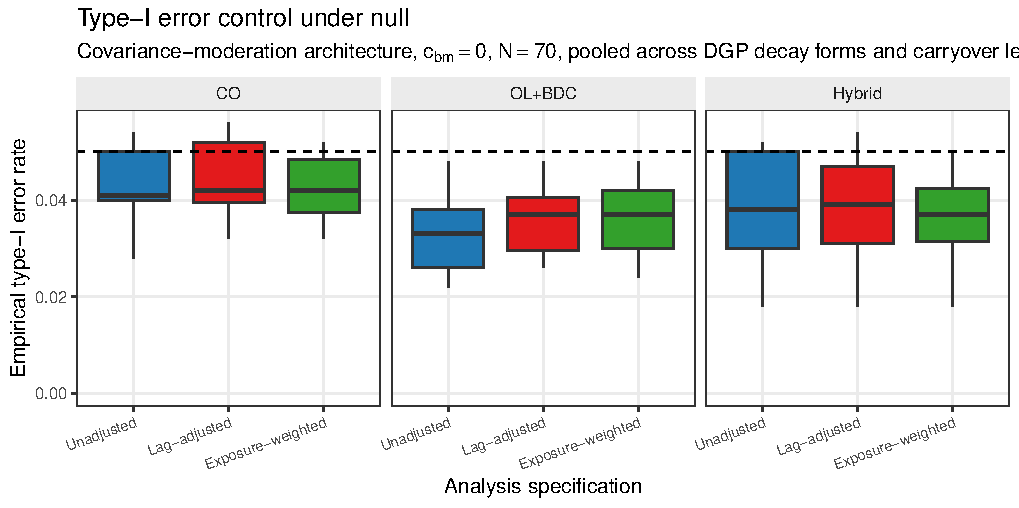
\includegraphics[width=0.8\linewidth]{../../figures/02xs-type1-boxplots} \caption{Empirical Type I error rates under the null ($c_{bm} = 0$), Architecture B, pooled across DGP decay forms and carryover half-lives, stratified by design and analysis specification. Boxplots cover the distribution across cells at $N = 70$; the dashed reference line marks the nominal 0.05 level.}\label{fig:fig-type1}
\end{figure}

Across the null cells, empirical Type I error sits uniformly below
the nominal 0.05 level for both specifications and in all three
designs. This shortfall is not sampling noise but a genuine
conservatism of the model-based interaction test, which the
companion calibration study\textsuperscript{\citeproc{ref-pmsimstats_calibration2026}{5}} traces to
the corCAR1 working covariance: the estimated standard error runs
six to ten percent too large, and the realized rejection rate falls
correspondingly. Because the conservatism is uniform across
specifications, it does not disturb the A2-versus-A3 comparison, and
the cluster-robust recalibration reported below (block S6) confirms
that a CR2 cluster-robust standard error restores the rejection rate
to nominal without changing which specification leads. Table
\ref{tab:tab-type1-cr2} makes the per-specification conservatism,
and its cluster-robust correction, explicit at the null cell.

\begin{table}

\caption{\label{tab:tab-type1-cr2}Conservatism of the model-based interaction test and its
    cluster-robust correction, at the null cell ($c_{bm} = 0$,
    exponential DGP, $t_{1/2} = 1.0$ weeks, Hybrid design, $N = 70$,
    Architecture B, 3{,}000 replicates). $\kappa$ is the ratio of the
    mean standard error to the empirical standard deviation of the
    interaction estimate; $\kappa > 1$ indicates a conservative
    test. Both specifications are conservative under the model-based
    test, most so the exposure-weighted A2 ($\kappa = 1.10$, Type I
    $= 0.029$); the CR2 bias-reduced cluster-robust standard error
    restores $\kappa$ to near one and Type I to nominal (0.045 to
    0.049) for both specifications.}
\centering
\begin{tabular}[t]{lllll}
\toprule
Specification & $\kappa$ model & Type I model & $\kappa$ CR2 & Type I CR2\\
\midrule
A2 & 1.10 & 0.029 & 1.00 & 0.045\\
A3 & 1.05 & 0.039 & 0.98 & 0.049\\
\bottomrule
\end{tabular}
\end{table}

\begin{table}
\centering
\caption{\label{tab:tab-s6}Cluster-robust recalibration of A2 (Power columns) and
    of the A2$-$A3 ranking (last two columns), at the reference cell
    and four stress cells (500 replicates, $c_{bm} = 0.45$,
    Architecture B). $\kappa$ is the ratio of the mean standard
    error to the empirical standard deviation of the interaction
    estimate for A2; a value above one is a conservative test. The
    A2$-$A3 columns are computed directly from the per-specification
    power at this cell under each inference, so they are a genuine
    check of this manuscript's own comparison rather than the
    A2-vs-A1 contrast reported for the full-scope grid. CR2 df is
    the mean Satterthwaite degrees of freedom for the cluster-robust
    test on A2. Computed with \texttt{clubSandwich}.}
\centering
\resizebox{\ifdim\width>\linewidth\linewidth\else\width\fi}{!}{
\begin{tabular}[t]{llllllll}
\toprule
Cell & $\kappa$ model & $\kappa$ CR2 & Power model & Power CR2 & A2$-$A3 model & A2$-$A3 CR2 & CR2 df\\
\midrule
Reference, $N=70$ & 1.15 & 0.99 & 0.829 & 0.863 & +0.082 & +0.090 & 23\\
Small $N=35$ & 1.13 & 0.96 & 0.558 & 0.590 & +0.068 & +0.086 & 12\\
High autocorr, $\rho=0.9$ & 1.26 & 0.94 & 0.954 & 0.980 & +0.052 & +0.036 & 23\\
Half-life mis-spec & 1.14 & 1.00 & 0.759 & 0.795 & +0.012 & +0.022 & 23\\
30\% MCAR dropout & 0.99 & 0.85 & 0.148 & 0.126 & +0.014 & -0.000 & 5\\
\bottomrule
\end{tabular}}
\end{table}

\begin{figure}
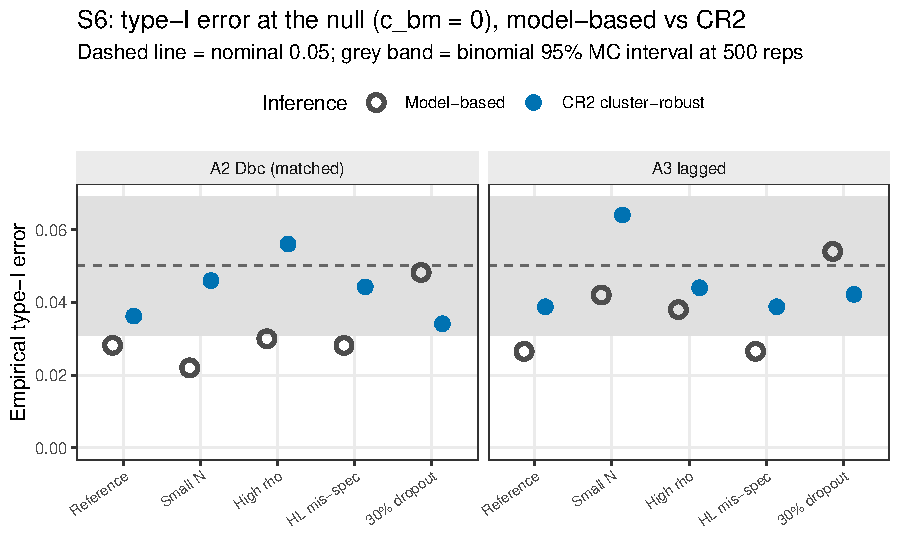
\includegraphics[width=0.8\linewidth]{../../figures/02xs-type1-cr2} \caption{Empirical Type I error at the null ($c_{bm} = 0$) under model-based and CR2 cluster-robust inference, across the five S6 stress cells and the two specifications (Architecture B). The model-based test (open) is conservative (near 0.03); CR2 (filled) is restored to the nominal 0.05 (dashed), within the binomial Monte Carlo band (gray). 500 null replicates per cell.}\label{fig:fig-type1-cr2}
\end{figure}

Figure \ref{fig:fig-type1-cr2} shows the effect of recalibration on
test size directly. The model-based null rejection rate sits below
nominal across all five S6 cells and both specifications, while the
CR2 test restores it to within the Monte Carlo band around 0.05.
This matters because a test that is not correctly sized cannot
fairly be preferred on power alone. In the information-rich cells,
the calibration ratio \(\kappa\) runs from 1.07 to 1.26 under the
model-based test and is restored to about one under CR2, and the
correctly sized test recovers two to five points of power in the
process. Table \ref{tab:tab-s6} reports the A2 minus A3 gap, which
is this manuscript's own comparison, computed directly from the
per-specification power at each S6 cell rather than borrowed from
the A2-versus-A1 contrast reported in the full-scope grid. That gap
is held or slightly widened under CR2 at the reference cell
(\(+0.080\) to \(+0.092\)), at the small-\(N\) cell (\(+0.068\) to
\(+0.086\)), and at the half-life mis-specification cell (\(+0.012\) to
\(+0.022\)); it narrows somewhat under high autocorrelation (\(+0.052\)
to \(+0.036\), though A2 still leads); and at 30\% MCAR dropout it
collapses from a small A2 lead under the model-based test
(\(+0.014\)) to an essentially null difference under CR2
(\(-0.0002\)), which we read as a statistical tie. We do not regard
this as a contradiction of the ranking so much as a restatement,
from a different angle, of the dropout finding in block S3 below:
A2's advantage is driven by information carried in the off-drug
observations, and once dropout has removed most of that information
there is not much left for either the model-based test or its
cluster-robust correction to distinguish. This recalibration was
validated only in the Architecture B, Hybrid, \(N = 70\) cells, and it
should not be extended to the crossover design, where A2 does not
lead in the first place.

\subsection{Sensitivity analyses}\label{sensitivity-analyses}

Four Tier 2 blocks perturb one axis at a time around a common
reference cell (Architecture B, Hybrid, \(N = 70\), \(c_{bm} = 0.45\),
exponential DGP, \(t_{1/2} = 1.0\)), holding the remaining factors
fixed. The blocks are reported separately here and are not pooled
with Tier 1 or with each other.

\subsubsection{S1: within-factor autocorrelation}\label{s1-within-factor-autocorrelation}

\begin{figure}
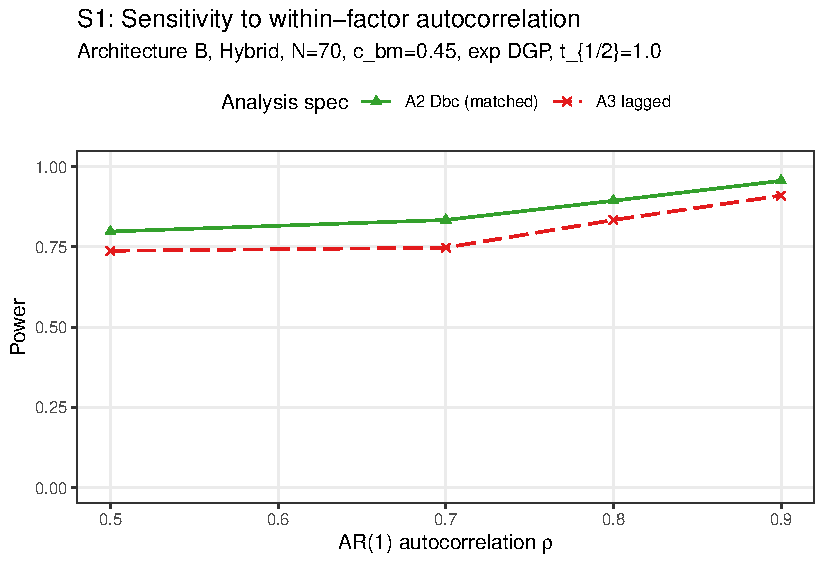
\includegraphics[width=0.6\linewidth]{../../figures/02xs-sens-S1} \caption{Power by analysis specification across AR(1) autocorrelation $\rho \in \{0.5, 0.7, 0.8, 0.9\}$, Architecture B.}\label{fig:fig-sens-s1}
\end{figure}

Both specifications gain power monotonically with \(\rho\). At
\(\rho = 0.5\), A2 power is \(0.798 \pm 0.018\) against A3's
\(0.738 \pm 0.020\); at \(\rho = 0.9\), A2 reaches \(0.956 \pm 0.009\)
against A3's \(0.910 \pm 0.013\) (point estimate plus or minus MCSE,
\(n_{sim} = 500\)). The A2 advantage over A3, roughly 0.06 in absolute
power throughout, is preserved at every autocorrelation level we
examined, which suggests that autocorrelation strength and the
choice of specification act additively rather than interacting with
one another.

\subsubsection{S2: analyst-truth half-life mismatch}\label{s2-analyst-truth-half-life-mismatch}

\begin{figure}
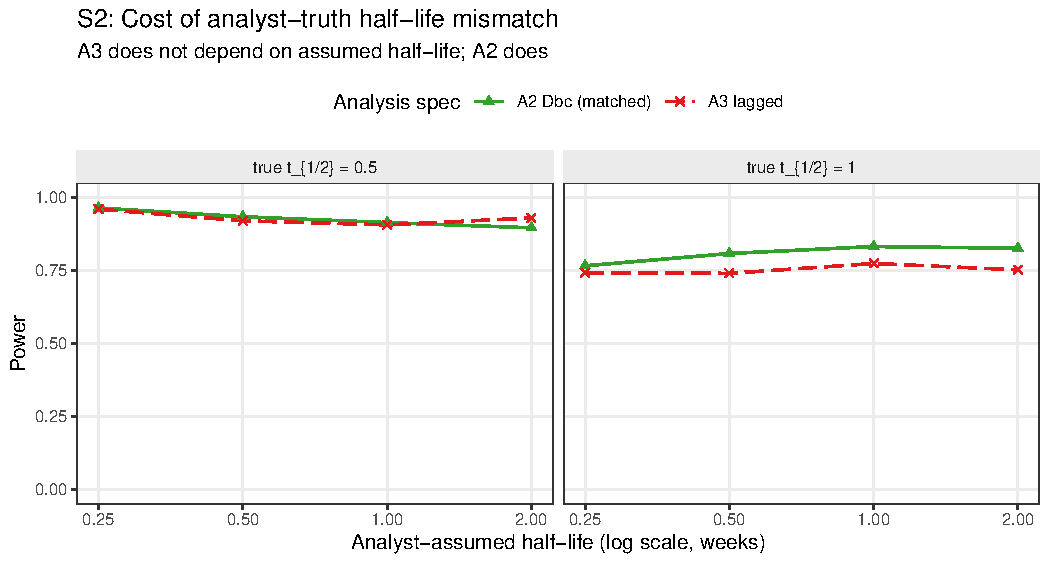
\includegraphics[width=0.8\linewidth]{../../figures/02xs-sens-S2} \caption{Power of A2 and A3 as the analyst's assumed half-life departs from the true DGP half-life. A3 is invariant to the assumed half-life by construction; A2's power degrades with mis-specification.}\label{fig:fig-sens-s2}
\end{figure}

A2 turns out to be fairly robust to a mismatch between the analyst's
assumed half-life and the true data-generating half-life. Across the
eight S2 cells (DGP \(t_{1/2} \in \{0.5, 1.0\}\) weeks crossed with
analyst-assumed \(t_{1/2} \in \{0.25, 0.5, 1.0, 2.0\}\) weeks), A2
averages 0.868, ranging from 0.766 to 0.964, with per-cell MCSE
between 0.008 and 0.019. A3, which does not consume the half-life
parameter, is invariant to the analyst's assumption by construction,
and its power averages 0.840 across the same eight cells. The
exposure-weighted predictor's curvature is gentle enough that
mis-specifying the assumed half-life by a factor of two does not
erode A2's advantage over A3 at either true half-life, which
suggests A2 remains a defensible choice even when the true
pharmacokinetic half-life is known only approximately at the design
stage.

\subsubsection{S3: dropout}\label{s3-dropout}

\begin{figure}
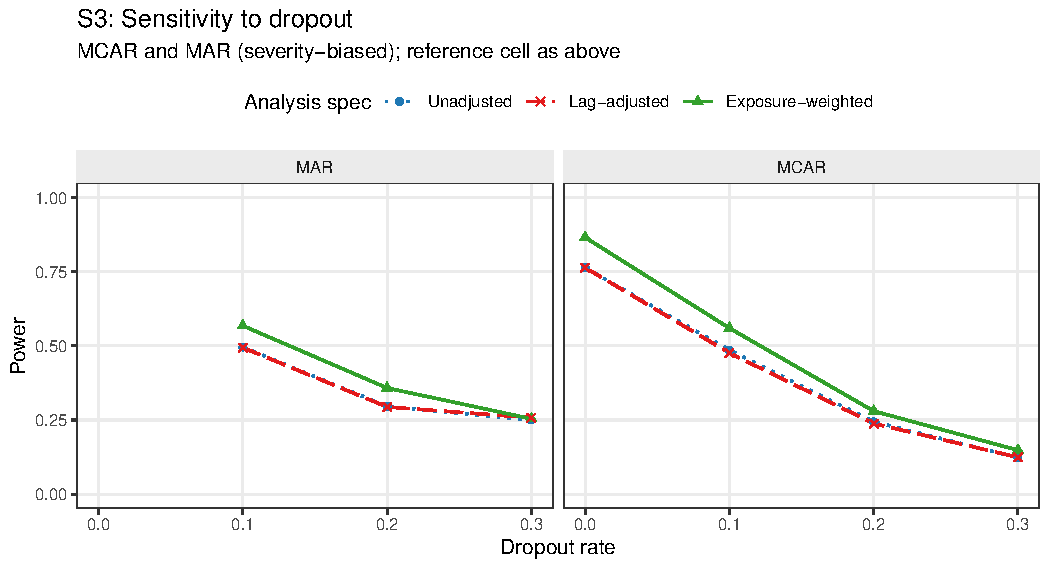
\includegraphics[width=0.8\linewidth]{../../figures/02xs-sens-S3} \caption{Power at dropout rates $\in \{0, 0.1, 0.2, 0.3\}$ under MCAR and MAR mechanisms, Architecture B.}\label{fig:fig-sens-s3}
\end{figure}

Both specifications lose power monotonically as the dropout rate
increases. At the MCAR baseline (\(N = 70\), no dropout), A2 gives
\(0.866 \pm 0.015\) and A3 gives \(0.764 \pm 0.019\); at an MCAR dropout
rate of 0.30, these collapse to \(0.148 \pm 0.016\) and
\(0.124 \pm 0.015\) respectively. A2's advantage narrows steadily as
dropout worsens: the absolute A2 minus A3 gap runs about 0.10 at
zero dropout, 0.07 at a rate of 0.10, 0.04 at 0.20, and 0.03 at 0.30
under MCAR, narrowing further under MAR dropout at the highest rate
examined (about 0.004 at rate 0.30). This pattern is consistent with
A2's advantage originating in the exposure-weighted contrast
contributed by off-drug observations; when those observations are
preferentially lost, A2's edge contracts toward A3's. At low to
moderate dropout, that is, at a rate of 0.20 or below, the A2
advantage is preserved.

\subsubsection{S4: biomarker-moderation effect-size curve}\label{s4-biomarker-moderation-effect-size-curve}

\begin{figure}
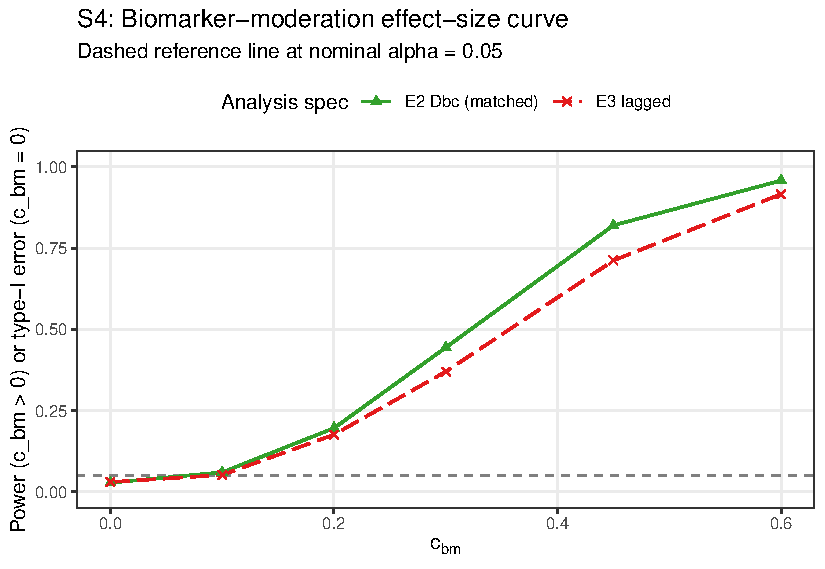
\includegraphics[width=0.6\linewidth]{../../figures/02xs-sens-S4} \caption{Power across the biomarker-moderation effect-size range $c_{bm} \in \{0, 0.10, 0.20, 0.30, 0.45, 0.60\}$ under Architecture B. The $c_{bm} = 0$ point is the null for Type I verification.}\label{fig:fig-sens-s4}
\end{figure}

The power curve is sigmoidal for both specifications, as expected.
At \(c_{bm} = 0\), empirical Type I error sits below nominal, at
\(0.028 \pm 0.007\) for A2 and \(0.030 \pm 0.008\) for A3; power then
rises through the mid-range and saturates once \(c_{bm} \geq 0.45\),
reaching \(0.958 \pm 0.009\) for A2 and \(0.916 \pm 0.012\) for A3 at
\(c_{bm} = 0.6\). The A2 advantage is largest at intermediate effect
sizes, \(+0.082\) absolute at \(c_{bm} = 0.30\) and \(+0.102\) at
\(c_{bm} = 0.45\), shrinking to \(+0.042\) at \(c_{bm} = 0.60\) as both
specifications approach the ceiling. The practical implication is
that the advantage matters most in trials targeting a moderate
biomarker-treatment interaction, and matters least when the true
effect is either very small or comfortably large.

\subsection{A higher-precision check}\label{a-higher-precision-check}

Because a number of the Tier 1 gaps are small, we reran a focused
24-cell grid (OL+BDC design, \(N \in \{35, 70\}\), true half-life
\(\in \{0.5, 1.0\}\)) at 600 trials per cell, with all trials
converging. Because A2 and A3 are fit to the same trials, we can
compare them with a paired McNemar test, which is considerably more
sensitive than treating the two specifications as independent
groups. Type I error across the twelve null cells of the rerun fell
in \([0.003, 0.053]\), so both specifications hold nominal alpha at
the sample sizes and half-lives examined. Paired McNemar tests on A2
versus A3 find A2 strictly ahead only at the highest-leverage cell
(\(N = 70\), true \(t_{1/2} = 1.0\) weeks, \(\Delta = +7.2\) percentage
points, \(p = 1.2 \times 10^{-7}\)); in the remaining three cells the
paired difference lies between \(-0.5\) and \(+1.5\) percentage points,
with \(p \geq 0.18\), and the two specifications are operationally
indistinguishable at this level of precision. Resolving the
A2-versus-A3 gap at the intermediate cells with statistical clarity
would require on the order of 2,000 replicates per cell, given the
current Monte Carlo standard error.

\section{Discussion}\label{discussion}

\subsection{The main result, and where it breaks down}\label{the-main-result-and-where-it-breaks-down}

The main finding is that A2's advantage over A3 is real, but
conditional. At its best cell (Hybrid design, \(N = 70\),
\(c_{bm} = 0.45\), \(t_{1/2} = 1.0\)), A2 beats A3 by about 10
percentage points of power (0.860 versus 0.770), a difference of
roughly five Monte Carlo standard errors and therefore not
attributable to chance. Under the crossover design, however, A2
does considerably worse (0.488 versus 0.830 for A3). The reason for
this reversal is not mysterious: in a crossover trial, the
within-subject correlation already carries most of the signal that
A2's decaying predictor was designed to recover, so A2 gains little
from its more elaborate representation of exposure, and its
down-weighting of off-drug observations simply works against it. The
ranking we would call `A2 is best' therefore holds only in the two
non-crossover designs studied here, and should not be extended to a
crossover trial.

\subsection{What the robustness checks add}\label{what-the-robustness-checks-add}

Three checks probe whether A2's advantage, where it exists, is
fragile. On decay shape (Figure \ref{fig:fig-heatmap-mismatch}):
even when the analyst wrongly assumes exponential decay and the true
form is Weibull, A2 still does not fall below A3, within the range
of decay shapes we examined. On the assumed half-life (Figure
\ref{fig:fig-sens-s2}): A3 does not use a half-life and is
therefore unaffected, while A2 does, yet getting the half-life wrong
by a factor of two or four moves A2's power only from about 0.83
down to 0.77, never below A3. On autocorrelation (Figure
\ref{fig:fig-sens-s1}): stronger serial correlation raises both
specifications by roughly the same amount, so A2's lead of five to
six points holds regardless of correlation strength. Taken together,
these checks suggest that where A2's advantage exists, it is not a
fragile artifact of one particular combination of nuisance
parameters.

\subsection{Dropout matters more than the method}\label{dropout-matters-more-than-the-method}

The most sobering finding in this study concerns missing data, not
carryover. When patients drop out (Figure \ref{fig:fig-sens-s3}),
power collapses for both specifications together: at 30\% dropout,
both fall to somewhere between 0.12 and 0.25 and become essentially
indistinguishable. A2 offers no protection against this loss; it can
only organize whatever data happen to remain. Dropout tied to
symptom severity (MAR) is somewhat worse than dropout occurring at
random (MCAR), because the sickest patients, who carry the most
signal, tend to leave first. The practical conclusion is blunt:
keeping patients in the trial buys considerably more statistical
power than the choice between A2 and A3 ever could.

\subsection{Scope, related work, and limits}\label{scope-related-work-and-limits}

This manuscript deliberately narrows the full-scope grid to
Architecture B, to the non-linear decay forms, and to the
A2-versus-A3 contrast, in the interest of bringing a thirty-page
evaluation down to a length a reviewer can reasonably read in one
sitting. The full-scope companion (report.Rmd and report-slim.Rmd)
shows that the A2 advantage documented here does not carry over to
Architecture A, where the biomarker moderates the mean response
directly and A2 is marginally dominated in every design we examined;
nor is the binary on-drug specification A1 dominated by A2 outside
the Hybrid and OL+BDC cells under Architecture B considered here.
Readers who need the cross-architecture comparison, or the
comparison against A1, should consult that manuscript rather than
extrapolate from this one.

Within the narrower scope adopted here, our matched-decay power at
the headline cell, \(0.860 \pm 0.016\), agrees with Hendrickson's\textsuperscript{\citeproc{ref-hendrickson2020}{2}} reported 0.82 for the same cell. The crossover
tradition represented by Jones and Kenward\textsuperscript{\citeproc{ref-jones2014crossover}{4}}
predicted that a shape-free lagged term such as A3 should outperform
a parametric predictor such as A2 once the decay shape is guessed
wrong; our S2 result does not support this expectation over the
range we examined, because A2's penalty for a wrong half-life turns
out to be too small for A3 to overtake it.

Two further limitations bound what we can conclude. First, the
numbers presented here come from a single parameter set, calibrated
to a prazosin and post-traumatic stress disorder trajectory, so the
absolute power values should be regarded as illustrative rather than
general; the ranking is the more portable part of the result, and
even the ranking is conditional on the trial design, as we have
shown above. Second, the sensitivity checks vary one factor at a
time and can therefore miss genuine interactions between factors,
for instance between high autocorrelation and heavy dropout; the one
joint check we are aware of, reported in the full-scope manuscript
as block S5, turned up no surprises.

\section{Conclusions}\label{conclusions}

\begin{enumerate}
\def\labelenumi{\arabic{enumi}.}
\item
  \textbf{A2 helps, but only under certain conditions.} The
  exposure-weighted predictor achieves the highest power, about 10
  points over A3, only in the Hybrid and OL+BDC designs, and its
  lead survives an incorrectly assumed decay shape and an
  incorrectly assumed half-life within those designs. Under the
  crossover design, A2 confers no advantage, and A3 is at least as
  good. Where A2 is used, we recommend reporting it with a CR2
  cluster-robust standard error (Block S6).
\item
  \textbf{A roughly guessed half-life is adequate, where A2 is used.}
  Getting the half-life wrong by a factor of two to four moves A2's
  power only modestly, so a rough pharmacokinetic estimate is
  sufficient in practice.
\item
  \textbf{Dropout matters more than either method.} Power falls sharply
  as dropout increases, roughly halving at a dropout rate of 20\%,
  and this loss affects both specifications equally. Preventing
  dropout is a more effective use of design effort than choosing
  between A2 and A3.
\item
  \textbf{The interaction test is somewhat conservative, and the problem
  is fixable.} Both specifications reject slightly less often than
  the nominal 5\% under the null, and a CR2 cluster-robust standard
  error restores the correct rate while recovering a modest amount
  of power. The A2-versus-A3 gap is held or widened under CR2 at
  four of the five S6 stress cells, but collapses to a statistical
  tie under 30\% dropout, consistent with the third conclusion above
  (Block S6).
\item
  \textbf{This is a narrowed slice of a larger study.} Architecture A,
  the binary specification A1, and linear decay all fall outside
  the scope of this manuscript; the full-scope grid reported in
  report.Rmd and report-slim.Rmd is the authority on those
  comparisons, and should be consulted before generalizing beyond
  Architecture B.
\end{enumerate}

\section*{Notes and reproducibility}\label{notes-and-reproducibility}
\addcontentsline{toc}{section}{Notes and reproducibility}

We declare no conflicts of interest and received no specific funding
for this work. This manuscript is a derivative of
report-extra-slim.Rmd, rewritten as continuous narrative; it
re-filters, but does not re-run, the same production simulation.
Cell-level summaries are available at
\texttt{analysis/data/02-grid-summary.rds} and
\texttt{02-sensitivity-summary.rds}; the filtered figures used here are
produced by \texttt{03-render-figures-extra-slim.R},
\texttt{04-sensitivity-figures-extra-slim.R}, and
\texttt{07-type1-cr2-figure-extra-slim.R} under
\texttt{analysis/scripts/carryover-sensitivity/}. No simulation code runs
during knitting. The production simulation ran under R 4.5.3, and
this document is rendered under R 4.6.0, both versions pinned via
\texttt{renv.lock}.

\section{References}\label{references}

\protect\phantomsection\label{refs}
\begin{CSLReferences}{0}{1}
\bibitem[\citeproctext]{ref-morris2019simulation}
\CSLLeftMargin{1. }%
\CSLRightInline{Morris TP, White IR, Crowther MJ. Using simulation studies to evaluate statistical methods. \emph{Statistics in Medicine}. 2019;38(11):2074-2102. doi:\href{https://doi.org/10.1002/sim.8086}{10.1002/sim.8086}}

\bibitem[\citeproctext]{ref-hendrickson2020}
\CSLLeftMargin{2. }%
\CSLRightInline{Hendrickson RC, Thomas RG, Schork NJ, Raskind MA. Optimizing aggregated {N}-of-1 trial designs for predictive biomarker validation: Statistical methods and practical considerations. \emph{Frontiers in Digital Health}. 2020;2:13. doi:\href{https://doi.org/10.3389/fdgth.2020.00013}{10.3389/fdgth.2020.00013}}

\bibitem[\citeproctext]{ref-pmsimstats_dgp_architectures2026}
\CSLLeftMargin{3. }%
\CSLRightInline{{pmsimstats team}. Two architectures for simulating biomarker-treatment interactions in aggregated {N}-of-1 trials. Published online 2026.}

\bibitem[\citeproctext]{ref-jones2014crossover}
\CSLLeftMargin{4. }%
\CSLRightInline{Jones B, Kenward MG. \emph{Design and Analysis of Cross-over Trials}. 3rd ed. CRC Press; 2014.}

\bibitem[\citeproctext]{ref-pmsimstats_calibration2026}
\CSLLeftMargin{5. }%
\CSLRightInline{{pmsimstats team}. Type-{I} calibration of fixed-effect interaction tests in linear mixed models: A staged diagnosis of working-covariance mis-specification and a cluster-robust remedy. Published online 2026.}

\end{CSLReferences}

\vfill

\begin{center}\rule{0.5\linewidth}{0.5pt}\end{center}

\emph{Rendered on 2026-07-10 at 00:29 AEST.}\\
\emph{Source: \texttt{\textasciitilde{}/prj/res/36-pmsimstats-ng/pmsimstats-ng/analysis/report/02-carryover-sensitivity/report-extra-slim-rgt.Rmd}}

\end{document}
